% Lecture notes: Week 10, Lecture 2 -- Principal Stresses, Failure, and Mohr's Circle
% To hide this lecture from the website, add a line containing only:  % draft
% To set the date shown on the website, add a line like:  % posted: 2026-09-02
\documentclass[11pt]{article}
\usepackage{mech2030notes}
\begin{document}

% ------------------------------------------------------------------
% Lecture-local helpers (defined inside the document so they also work
% in the combined notes; names are unique to this lecture).
%
% \WTenLTwoMohr{n}: draws the example's Mohr's circle as it looks after
% step n of the procedure, with the piece added at step n in red.
% Scale: 1 unit = 100 MPa; tau is plotted positive DOWNWARD.
%   A = (sigma_x, tau_xy) = (300, 100)      -> (3, -1)
%   G = (sigma_y, -tau_xy) = (-200, -100)   -> (-2, 1)
%   C = (sigma_avg, 0) = (50, 0)            -> (0.5, 0),  R = 2.6926
% ------------------------------------------------------------------
\newcommand{\WTenLTwoCol}[2]{\ifnum#1=#2\def\wtlc{red!75!black}\else\def\wtlc{black}\fi}
\newcommand{\WTenLTwoMohr}[1]{%
  \ifnum#1>1
    \WTenLTwoCol{#1}{2}%
    \draw[axis, \wtlc] (-3.2,0) -- (4.0,0) node[right] {$\sigma$};
    \draw[axis, \wtlc] (0,3.0) -- (0,-3.2) node[below] {$\tau$};
    \foreach \s in {-2,-1,1,2,3} \draw[thin, \wtlc] (\s,0.07) -- (\s,-0.07);
  \fi
  \ifnum#1>5
    \WTenLTwoCol{#1}{6}%
    \draw[semithick, \wtlc] (0.5,0) circle (2.6926);
  \fi
  \ifnum#1>4
    \WTenLTwoCol{#1}{5}%
    \draw[thick, \wtlc] (-2,1) -- (3,-1);
    \node[pin, \wtlc] at (0.5,0) {};
    \node[above right, \wtlc] at (0.45,0.02) {$\sigma_{\text{avg}}$};
  \fi
  \ifnum#1>2
    \WTenLTwoCol{#1}{3}%
    \node[pin, \wtlc] at (3,-1) {};
    \node[right, \wtlc] at (3.05,-1.05) {$A\,(\sigma_x, \tau_{xy})$};
  \fi
  \ifnum#1>3
    \WTenLTwoCol{#1}{4}%
    \node[pin, \wtlc] at (-2,1) {};
    \node[above left, \wtlc] at (-2,1) {$G\,(\sigma_y, -\tau_{xy})$};
  \fi
  \ifnum#1>6
    \WTenLTwoCol{#1}{7}%
    \draw[thick, \wtlc] (0.5,0) -- (0.5,-2.6926);
    \node[pin, \wtlc] at (0.5,-2.6926) {};
    \node[below, \wtlc] at (0.5,-2.6926) {$\tau_{\max}$};
    \node[right, \wtlc] at (0.5,-2.3) {$R$};
  \fi
  \ifnum#1>7
    \WTenLTwoCol{#1}{8}%
    \node[pin, \wtlc] at (3.1926,0) {}; \node[above right, \wtlc] at (3.15,0) {$\sigma_1$};
    \node[pin, \wtlc] at (-2.1926,0) {}; \node[above left, \wtlc] at (-2.15,0) {$\sigma_2$};
  \fi
  \ifnum#1>8
    \WTenLTwoCol{#1}{9}%
    \draw[thinarrow, \wtlc] (0.5,0) ++(-21.8:1.5) arc (-21.8:0:1.5);
    \node[\wtlc] at ($(0.5,0)+(-10:2.15)$) {$2\theta_{p1}$};
    \draw[thinarrow, \wtlc] (0.5,0) ++(-21.8:0.55) arc (-21.8:-180:0.55);
    \node[\wtlc] at ($(0.5,0)+(-163:1.45)$) {$2\theta_{p2}$};
  \fi
  \ifnum#1>9
    \WTenLTwoCol{#1}{10}%
    \draw[thinarrow, \wtlc] (0.5,0) ++(-21.8:1.85) arc (-21.8:-90:1.85);
    \node[\wtlc] at ($(0.5,0)+(-58:2.25)$) {$2\theta_s$};
  \fi
}

% ##################################################################
%  WEEK 10, LECTURE 2
% ##################################################################
\lecture{10}{2}{Principal Stresses, Failure, and Mohr's Circle}

% ==================================================================
\section*{Recap: Stress Transformations}
% ==================================================================

\noindent
\begin{minipage}[c]{0.5\textwidth}
\centering
\begin{tikzpicture}
  \dogbone{0}{0.3}{1.0}
  \draw[force] (0,2.55) -- (0,3.2) node[right] {$P$};
  \draw[force] (0,-2.55) -- (0,-3.2) node[right] {$P$};
  % small element in the gauge section and zoom lines
  \draw[thin, fill=gray!40] (0,0.38) -- (0.18,0.2) -- (0,0.02) -- (-0.18,0.2) -- cycle;
  \draw[thin] (0.18,0.2) -- (2.1,0.95);
  \draw[thin] (0.18,0.2) -- (2.1,-0.55);
  % zoomed 45-degree element: pure shear converging on the top and bottom corners
  \draw[thick, fill=gray!20] (3,1.1) -- (3.9,0.2) -- (3,-0.7) -- (2.1,0.2) -- cycle;
  \draw[-{Stealth[length=2mm,width=1.5mm]}, thick, red!70!black]
       ($(2.1,0.2)!0.2!(3,1.1)+(-0.15,0.15)$) -- ($(2.1,0.2)!0.85!(3,1.1)+(-0.15,0.15)$);
  \draw[-{Stealth[length=2mm,width=1.5mm]}, thick, red!70!black]
       ($(3.9,0.2)!0.2!(3,1.1)+(0.15,0.15)$) -- ($(3.9,0.2)!0.85!(3,1.1)+(0.15,0.15)$);
  \draw[-{Stealth[length=2mm,width=1.5mm]}, thick, red!70!black]
       ($(2.1,0.2)!0.2!(3,-0.7)+(-0.15,-0.15)$) -- ($(2.1,0.2)!0.85!(3,-0.7)+(-0.15,-0.15)$);
  \draw[-{Stealth[length=2mm,width=1.5mm]}, thick, red!70!black]
       ($(3.9,0.2)!0.2!(3,-0.7)+(0.15,-0.15)$) -- ($(3.9,0.2)!0.85!(3,-0.7)+(0.15,-0.15)$);
  \node[right] at (3.55,0.95) {$\tau$};
  % the applied tension, shown on reference lines above and below
  \draw[thin] (2.3,1.45) -- (3.7,1.45);
  \draw[force] (3,1.45) -- (3,2.05) node[above] {$\sigma$};
  \draw[thin] (2.3,-1.05) -- (3.7,-1.05);
  \draw[force] (3,-1.05) -- (3,-1.65) node[below] {$\sigma$};
\end{tikzpicture}
\end{minipage}%
\hfill
\begin{minipage}[c]{0.46\textwidth}
Last time, we saw that \emph{uniaxial tension} in one coordinate system actually creates
\emph{shear stress} in another coordinate system (rotated by $\ang{45}$).

\medskip
{\small (The $45^\circ$ element also carries normal stresses $\sigma/2$ on every face,
omitted here for clarity; see Week~10, Lecture~1.)}
\end{minipage}

\bigskip
\begin{itemize}
  \item In fact, \emph{any} 2D stress state $(\sigma_x, \sigma_y, \tau_{xy})$ can be rotated
        by an angle $\theta$ to get another, equivalent stress state
        $(\sigma_{x'}, \sigma_{y'}, \tau_{x'y'})$.
  \begin{itemize}[label=--]
    \item This rotation of the stress state is the definition of a
          \emph{stress transformation}.
  \end{itemize}
  \item The highest and lowest possible values of $\sigma_{x'}$ are the
        \emph{principal stresses}
        \[
          (\sigma_1, \sigma_2) \quad\text{with}\quad \sigma_1 > \sigma_2,
          \qquad\text{with orientations}\quad (\theta_{p1}, \theta_{p2}).
        \]
  \item The highest possible magnitude of $\tau_{x'y'}$ is the \emph{max shear}
        \[
          \tau_{\max} \quad\text{with orientation}\quad \theta_s.
        \]
\end{itemize}

% ==================================================================
\section*{Why Principal Values Matter: Material Failure}
% ==================================================================

\noindent
These quantities, $(\sigma_1, \sigma_2, \tau_{\max})$, are very important for
engineering analysis, because they control how materials \emph{fail}.

\begin{center}
\begin{minipage}[t]{0.45\textwidth}
\centering
\textbf{Brittle} (e.g.\ concrete)\\[0.6em]
\begin{tikzpicture}
  % cylinder in tension with a flat crack perpendicular to the load
  \fill[gray!12] (-0.7,-1.6) rectangle (0.7,1.6);
  \draw[thick] (-0.7,-1.6) -- (-0.7,1.6) (0.7,-1.6) -- (0.7,1.6);
  \draw[thick, fill=gray!25] (0,1.6) ellipse (0.7 and 0.18);
  \draw[thick] (-0.7,-1.6) arc (180:360:0.7 and 0.18);
  \draw[very thick] (-0.7,0.04) -- (-0.45,-0.06) -- (-0.2,0.07) -- (0.05,-0.05)
                    -- (0.3,0.06) -- (0.5,-0.04) -- (0.7,0.03);
  \draw[force] (0,1.8) -- (0,2.45) node[right] {$P$};
  \draw[force] (0,-1.8) -- (0,-2.45) node[right] {$P$};
  % sigma_1 pulling the crack faces apart
  \draw[force, red!70!black] (1.1,0.15) -- (1.1,0.85);
  \draw[force, red!70!black] (1.1,-0.15) -- (1.1,-0.85);
  \node[right, red!70!black] at (1.15,0.5) {$\sigma_1$};
  \node[left, font=\small] at (-0.8,0) {crack};
\end{tikzpicture}
\end{minipage}%
\hfill
\begin{minipage}[t]{0.5\textwidth}
\centering
\textbf{Ductile} (e.g.\ aluminum)\\[0.6em]
\begin{tikzpicture}
  \dogbone{0}{0.3}{1.0}
  \draw[force] (0,2.55) -- (0,3.2) node[right] {$P$};
  \draw[force] (0,-2.55) -- (0,-3.2) node[right] {$P$};
  % slanted shear band in the gauge section, with zoom
  \fill[gray!55] (-0.3,-0.36) -- (0.3,0.24) -- (0.3,0.36) -- (-0.3,-0.24) -- cycle;
  \draw[thin] (-0.36,-0.42) rectangle (0.36,0.42);
  \draw[thin] (0.36,0.42) -- (1.4,0.9);
  \draw[thin] (0.36,-0.42) -- (1.4,-0.9);
  \begin{scope}[shift={(2.3,0)}]
    \fill[gray!12] (-0.9,-0.9) rectangle (0.9,0.9);
    \fill[gray!55] (-0.9,-1.0+0.1) -- (0.9,0.8) -- (0.9,1.0-0.1+0.1) -- (-0.9,-0.8+0.1) -- cycle;
    \draw[thin] (-0.9,-0.9) rectangle (0.9,0.9);
    \draw[-{Stealth[length=2mm,width=1.5mm]}, thick, red!70!black] (-0.75,-0.25) -- (0.1,0.6);
    \draw[-{Stealth[length=2mm,width=1.5mm]}, thick, red!70!black] (0.75,0.25) -- (-0.1,-0.6);
    \node[red!70!black, fill=white, inner sep=1pt] at (0.55,-0.55) {$\tau_{\max}$};
  \end{scope}
\end{tikzpicture}
\end{minipage}
\end{center}

\begin{itemize}
  \item \emph{Brittle} materials like concrete fail when
        \[ \boxed{\sigma_1 > \sigma_{1,\text{cr}}} \]
        and the crack path is \emph{perpendicular} to the $\theta_{p1}$ direction
        (the crack faces are pulled apart by $\sigma_1$).
  \item \emph{Ductile} materials like aluminum fail along the direction of
        \emph{max shear}:
        \[ \boxed{\tau_{\max} \text{ oriented at } \theta_s} \]
\end{itemize}

\noindent
$\rightarrow$ For the uniaxial tension test above ($\sigma_x = 0$, $\sigma_y = \sigma$,
$\tau_{xy} = 0$):
\begin{itemize}[label=\then]
  \item $\sigma_1 = \sigma$ acts along the load ($\theta_{p1} = \ang{0}$ from the loading
        axis), so a brittle specimen cracks \emph{straight across}.
  \item $\tau_{\max} = \sigma/2$ acts on planes at $\ang{45}$ to the load, so a ductile
        specimen fails along a \emph{slanted} band.
\end{itemize}


% ==================================================================
\section*{Mohr's Circle: Example Problem}
% ==================================================================

\noindent
\begin{minipage}[c]{0.55\textwidth}
\textbf{Setup:} A stress state is shown for a piece of solid material.

\smallskip
\textbf{Find:} For this stress state, use Mohr's circle to determine:
\begin{enumerate}[label=(\alph*)]
  \item the average normal stress $\sigma_{\text{avg}}$,
  \item the principal stresses $\sigma_1$ and $\sigma_2$ and their associated orientations
        $\theta_{p1}$ and $\theta_{p2}$, and
  \item the maximum in-plane shear stress $\tau_{\max}$ and its associated orientation
        $\theta_s$.
\end{enumerate}
\end{minipage}%
\hfill
\begin{minipage}[c]{0.42\textwidth}
\centering
\begin{tikzpicture}
  \draw[thick, fill=gray!12] (-0.8,-0.8) rectangle (0.8,0.8);
  % sigma_x = +300 MPa (tension)
  \draw[force] (0.85,0) -- (1.6,0) node[right] {$\SI{300}{MPa}$};
  \draw[force] (-0.85,0) -- (-1.6,0);
  % sigma_y = -200 MPa (compression: arrows point INTO the element)
  \draw[force] (0,1.6) node[above] {$\SI{200}{MPa}$} -- (0,0.85);
  \draw[force] (0,-1.6) -- (0,-0.85);
  % tau_xy = +100 MPa
  \draw[force] (1.0,-0.55) -- (1.0,0.55);
  \draw[force] (-1.0,0.55) -- (-1.0,-0.55);
  \draw[force] (-0.55,1.0) -- (0.55,1.0) node[right] {$\SI{100}{MPa}$};
  \draw[force] (0.55,-1.0) -- (-0.55,-1.0);
\end{tikzpicture}
\end{minipage}

\subsection*{Building Mohr's circle, step by step}

\noindent
Each panel shows the circle after that step; the piece added in the current step is in
\textcolor{red!75!black}{red}. (Scale: one tick $= \SI{100}{MPa}$.)

\newcommand{\WTenLTwoPanel}[1]{%
  \begin{tikzpicture}[scale=0.7, every node/.style={font=\scriptsize}]
    \WTenLTwoMohr{#1}
  \end{tikzpicture}}

\medskip
\noindent
\begin{minipage}[c]{0.55\textwidth}
\textbf{1. What are $\sigma_x$, $\sigma_y$, and $\tau_{xy}$?}
\begin{itemize}
  \item $\sigma_x = +\SI{300}{MPa}$ (tension)
  \item $\sigma_y = -\SI{200}{MPa}$ (\emph{compression}: the arrows point into the faces)
  \item $\tau_{xy} = +\SI{100}{MPa}$ (up on the $+x$ face, right on the $+y$ face)
\end{itemize}
\end{minipage}%
\hfill
\begin{minipage}[c]{0.42\textwidth}
\centering
\textit{(no drawing yet)}
\end{minipage}

\bigskip
\noindent
\begin{minipage}[c]{0.53\textwidth}
\textbf{2. Draw the axes.}
\begin{itemize}
  \item Horizontal axis: $\sigma$ (positive to the right).
  \item Vertical axis: $\tau$, plotted positive \emph{downward}.
\end{itemize}
\end{minipage}%
\hfill
\begin{minipage}[c]{0.44\textwidth}
\centering\WTenLTwoPanel{2}
\end{minipage}

\bigskip
\noindent
\begin{minipage}[c]{0.53\textwidth}
\textbf{3. Draw a dot at the point $(\sigma_x, \tau_{xy})$.}
\[ A = (300,\ 100)\ \si{MPa} \]
This point represents the $x$-face of the element, i.e.\ $\theta = \ang{0}$.
\end{minipage}%
\hfill
\begin{minipage}[c]{0.44\textwidth}
\centering\WTenLTwoPanel{3}
\end{minipage}

\bigskip
\noindent
\begin{minipage}[c]{0.53\textwidth}
\textbf{4. Draw a dot at the point $(\sigma_y, -\tau_{xy})$.}
\[ G = (-200,\ -100)\ \si{MPa} \]
This point represents the $y$-face of the element.
\end{minipage}%
\hfill
\begin{minipage}[c]{0.44\textwidth}
\centering\WTenLTwoPanel{4}
\end{minipage}

\bigskip
\noindent
\begin{minipage}[c]{0.53\textwidth}
\textbf{5. Draw a line between the two dots.} Where it crosses the $\sigma$-axis is
$\sigma_{\text{avg}}$:
\[
  \sigma_{\text{avg}} = \frac{\sigma_x + \sigma_y}{2} = \frac{300 - 200}{2}
\]
\[ \boxed{\sigma_{\text{avg}} = \SI{50}{MPa}} \]
\end{minipage}%
\hfill
\begin{minipage}[c]{0.44\textwidth}
\centering\WTenLTwoPanel{5}
\end{minipage}

\bigskip
\noindent
\begin{minipage}[c]{0.53\textwidth}
\textbf{6. Draw the circle} centered at $(\sigma_{\text{avg}}, 0)$ and passing through the
points from steps 3 and 4.
\begin{itemize}[label=\then]
  \item \emph{Every} point on the circle is an equivalent stress state, for some rotation
        $\theta$.
\end{itemize}
\end{minipage}%
\hfill
\begin{minipage}[c]{0.44\textwidth}
\centering\WTenLTwoPanel{6}
\end{minipage}

\bigskip
\noindent
\begin{minipage}[c]{0.53\textwidth}
\textbf{7. What is the radius of the circle?} This radius is $\tau_{\max}$:
\begin{align*}
  R = \tau_{\max} &= \sqrt{\left(\frac{\sigma_x - \sigma_y}{2}\right)^2 + \tau_{xy}^2} \\
  &= \sqrt{(250)^2 + (100)^2}
\end{align*}
\[ \boxed{R = \tau_{\max} = \SI{269}{MPa}} \]
\end{minipage}%
\hfill
\begin{minipage}[c]{0.44\textwidth}
\centering\WTenLTwoPanel{7}
\end{minipage}

\bigskip
\noindent
\begin{minipage}[c]{0.53\textwidth}
\textbf{8. What are the max and min axial stresses on the circle?} These are $\sigma_1$
and $\sigma_2$:
\begin{align*}
  \sigma_1 &= \sigma_{\text{avg}} + R = 50 + 269 = \boxed{\SI{319}{MPa}} \\
  \sigma_2 &= \sigma_{\text{avg}} - R = 50 - 269 = \boxed{-\SI{219}{MPa}}
\end{align*}
\end{minipage}%
\hfill
\begin{minipage}[c]{0.44\textwidth}
\centering\WTenLTwoPanel{8}
\end{minipage}

\bigskip
\noindent
\begin{minipage}[c]{0.53\textwidth}
\textbf{9. What are the two angles between the drawn diameter and the $\sigma$-axis?}
These angles are $2\theta_{p1}$ and $2\theta_{p2}$:
\[
  \tan(2\theta_{p1}) = \frac{\tau_{xy}}{\tfrac12(\sigma_x - \sigma_y)} = \frac{100}{250}
\]
\[
  \theta_{p1} = \tfrac12\tan^{-1}(0.4)
\]
\[ \boxed{\theta_{p1} = \ang{10.9}} \quad \text{(counterclockwise, positive)} \]
Graphically, $|2\theta_{p1}| + |2\theta_{p2}| = \ang{180}$, so
$|\theta_{p2}| = \ang{90} - |\theta_{p1}| = \ang{79.1}$:
\[ \boxed{\theta_{p2} = -\ang{79.1}} \quad \text{(clockwise, negative)} \]
\end{minipage}%
\hfill
\begin{minipage}[c]{0.44\textwidth}
\centering\WTenLTwoPanel{9}
\end{minipage}

\bigskip
\noindent
\begin{minipage}[c]{0.53\textwidth}
\textbf{10. What is the angle between the drawn diameter and the vertical direction?}
This angle is $2\theta_s$:

\smallskip
$|2\theta_s| + |2\theta_{p1}| = \ang{90}$, so
$|\theta_s| = \ang{45} - |\theta_{p1}| = \ang{34.1}$:
\[ \boxed{\theta_s = -\ang{34.1}} \quad \text{(clockwise, negative)} \]
\end{minipage}%
\hfill
\begin{minipage}[c]{0.44\textwidth}
\centering\WTenLTwoPanel{10}
\end{minipage}

\subsection*{Completed circle}

\begin{center}
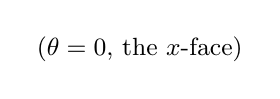
\begin{tikzpicture}[scale=1.0, every node/.style={font=\small}]
  \WTenLTwoMohr{11}
  \node[below right, font=\small] at (3.05,-1.3) {($\theta = \ang{0}$, the $x$-face)};
\end{tikzpicture}
\end{center}

\subsection*{Summary}

\noindent
\begin{minipage}[t]{0.48\textwidth}
\textbf{Mohr's circle formulas:}
\begin{align*}
  \sigma_{\text{avg}} &= \frac{\sigma_x + \sigma_y}{2} \\
  R = \tau_{\max} &= \sqrt{\left(\frac{\sigma_x - \sigma_y}{2}\right)^2 + \tau_{xy}^2} \\
  \sigma_1 &= \sigma_{\text{avg}} + R \\
  \sigma_2 &= \sigma_{\text{avg}} - R
\end{align*}
\end{minipage}%
\hfill
\begin{minipage}[t]{0.48\textwidth}
\textbf{Solution:}\\[0.6em]
\fbox{\fbox{\begin{tabular}{l @{\qquad} l}
  $\sigma_{\text{avg}} = \SI{50}{MPa}$ & \\[2pt]
  $\sigma_1 = \SI{319}{MPa}$ & $\theta_{p1} = \ang{10.9}$ \\[2pt]
  $\sigma_2 = -\SI{219}{MPa}$ & $\theta_{p2} = -\ang{79.1}$ \\[2pt]
  $\tau_{\max} = \SI{269}{MPa}$ & $\theta_s = -\ang{34.1}$
\end{tabular}}}
\end{minipage}

\end{document}
